Lo scopo di questa seconda esperienza è realizzare un generatore di onda triangolare, quadra e sinusoidale basato su un multi vibratore astabile, secondo lo schema riportato in Figura \ref{fig:Circuit2}. Sono stati utilizzati i seguenti componenti:
\begin{itemize}
    \item Amplificatore operazionale, codice TL082CP
    \item Resistenze $R_1=10\text{k}\Omega$, da 0.25W 
    \item Resistenza $R_2=39\text{k}\Omega$, da 0.25W 
    \item Resistenza $R$, da calcolare
    \item Condensatore $C$, da scegliere tra i disponibili.
\end{itemize}
\begin{figure}[H]
    \centering
    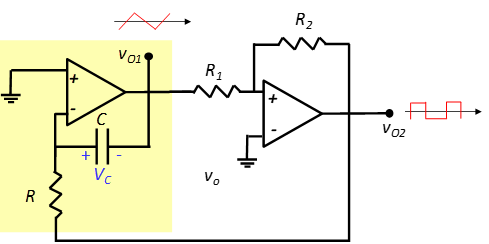
\includegraphics[width=0.65\linewidth]{images/Circuit2.png}
    \caption{Schema circuito}
    \label{fig:Circuit2}
\end{figure}
Il circuito è alimentato dalla tensione duale: $\pm V_{CC}=\pm 10V$.
\subsection{PRELAB}
Sono stati determinati i valori delle soglie $V_{TH}$ e $V_{TL}$ dalle condizioni operative determinate nel primo esperimento
\begin{table}[H]
    \centering
    \begin{tabular}{|c|c|}
        \hline
        $V_{TH}=$& $-L_-(R_1/R_2)=2.2154V$  \\\hline
        $V_{TL}=$& $-L_+(R_1/R_2)=-2.35V$ \\\hline
    \end{tabular}
    %\caption{Soglie di funzionamento del circuito}
    %\label{tab:my_label}
\end{table}
In seguito sono stati scelti i valori di $R$ e $C$ in modo da ottenere frequenza di oscillazione pari a $f=1kHz\pm10\%$
\begin{table}[H]
    \centering
    \begin{tabular}{|c|c|}
        \hline
        $R=$& $10k\Omega$ \\\hline
        $C=$& $100nF$ \\\hline
    \end{tabular}
    %\caption{Soglie di funzionamento del circuito}
    %\label{tab:my_label}
    
\end{table}
I valori di $R$ e $C$ sono stati ottenuti con la seguente formula
\begin{equation}
    T = \frac{1}{f} = \frac{2RC(V_{TH}-V_{TL})}{L_+}
\end{equation}
\subsection{Risultati}
Si realizza il circuito in Figura \ref{fig:Circuit2} connettendo l'oscilloscopio alle uscite $v_{01} \text{ e }v_{02}$ e si accendono le uscite dell'alimentatore $\pm V_{CC}=\pm 10V$. L'oscilloscopio è stato impostato in modo tale da visualizzare simultaneamente i segnali $v_{01} \text{ e }v_{02}$, come è stato riportato in Figura \ref{fig:Ris2}.
\begin{figure}[H]
    \centering
    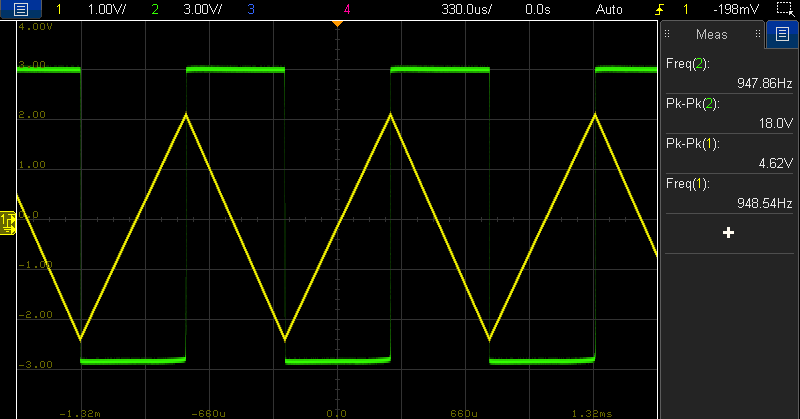
\includegraphics[width=0.7\linewidth]{images/scope_11.png}
    \caption{Forme d'onda dei segnali $v_{01} \text{ e }v_{02}$}
    \label{fig:Ris2}
\end{figure}
Successivamente sono state misurati i parametri delle forme d'onda $v_{01} \text{ e }v_{02}$ e riportati in Tabella \ref{tab:Ris2}
\begin{table}[H]
    \centering
    \begin{tabular}{||c|c|c||}
        \hline
        Segnale&Ampiezza picco-picco&Frequenza \\\hline\hline
        $v_{01}$&$Pk-Pk(1)=4.47V$&$F(1)=947.98Hz$\\\hline
        $v_{02}$&$Pk-Pk(2)=17.58V$&$F(2)=947.83Hz$\\\hline
    \end{tabular}
    \caption{Misure delle forme d'onda $v_{01} \text{ e }v_{02}$}
    \label{tab:Ris2}
\end{table}
\clearpage
\subsection{Generatore onda sinusoidale}
Volendo generare anche un'onda sinusoidale, viene collegato un filtro passa-basso all'uscita $v_{01}$, come riportato in Figura \ref{fig:Circuit2.1}.
\begin{figure}[H]
    \centering
    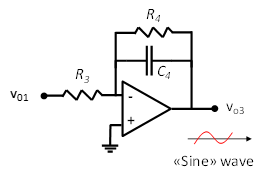
\includegraphics{images/Circuit2.1.png}
    \caption{Schema circuito}
    \label{fig:Circuit2.1}
\end{figure}
\subsubsection{Scelta dei valori di $R_3$ e $R_4$ - prelab}
Sono stati scelti i valori delle resistenze, usando $C=100nF$ in modo da ottenere frequenza di taglio pari a $100Hz$ e guadagno unitario in bassa frequenza
\begin{table}[H]
    \centering
    \begin{tabular}{|c|c|}
        \hline
        $R_3=$& $16k\Omega$  \\\hline
        $R_4=$& $16k\Omega$  \\\hline
        $C=$& $100nF$ \\\hline
    \end{tabular}
    %\caption{Soglie di funzionamento del circuito}
    %\label{tab:my_label}
\end{table}
Il dimensionamento delle resistenze del circuito affinché il filtro passa-basso abbia guadagno unitario in bassa frequenza e frequenza di taglio pari a 100Hz è il seguente. Dalla funzione di trasferimento del filtro si ottiene 
\begin{equation}
    A_0=\frac{R_3}{R_4}=1\implies R_3=R_4
\end{equation}
Dalla frequenza di taglio si ricava il valore delle resistenze
\begin{equation}
    F=\frac{1}{2\pi R_4C}=100Hz\implies R_3=R_4=\frac{1}{2\pi CF}\approx16k\Omega
\end{equation}
\clearpage
\subsubsection{Risultati}
Dopo aver realizzato il circuito e collegato l'ingresso all'uscita $v_{01}$. Sull'oscilloscopio sono state visualizzate le forme d'onda $v_{01}\text{ e }v_{03}$, che sono riportate in Figura \ref{fig:Ris2.1}.
\begin{figure}[H]
    \centering
    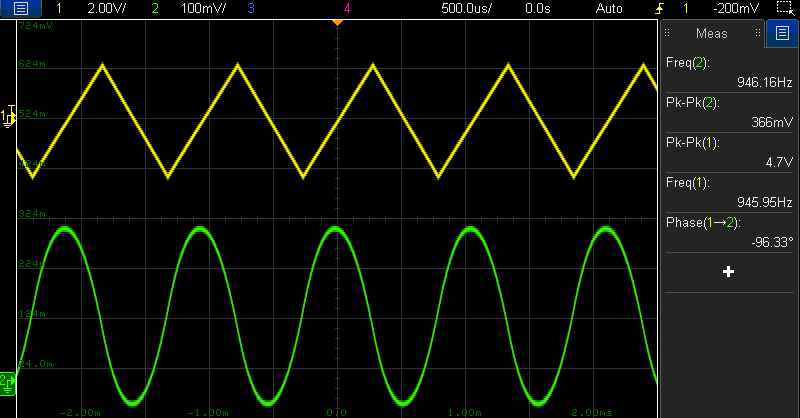
\includegraphics[width=0.6\linewidth]{images/scope_12.png}
    \caption{Forme d'onda $v_{01}\text{ e }v_{03}$}
    \label{fig:Ris2.1}
\end{figure}
Inoltre sono stati misurati l'ampiezza picco-picco della sinusoide generata e lo sfasamento rispetto all'onda triangolare generata, riportata in Tabella \ref{tab:Ris2.1}
\begin{table}[H]
    \centering
    \begin{tabular}{||c|c||}
        \hline
        Ampiezza picco-picco&$303mV$\\\hline
        Fase&-95.686°\\\hline
    \end{tabular}
    \caption{Misurazioni sulle forme d'onda $v_{01}\text{ e }v_{03}$}
    \label{tab:Ris2.1}
\end{table}
Infine è stata messa a confronto l'onda sinusoidale generata dal circuito con quella generata dal generatore di funzione impostato sugli stessi parametri. In Figura \ref{fig:Ris2.2} sono riportate le due forme d'onda
\begin{figure}[H]
    \centering
    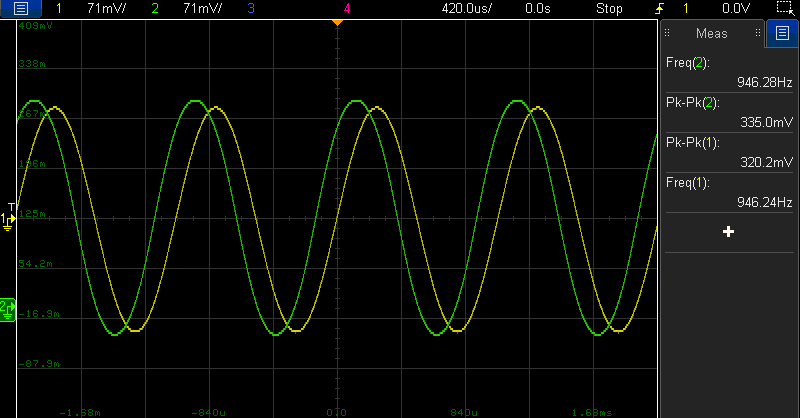
\includegraphics[width=0.6\linewidth]{images/scope_15.png}
    \caption{Forma d'onda generata dal circuito e "pura"}
    \label{fig:Ris2.2}
\end{figure}
Possiamo notare che le due forme d'onda sono pressoché identiche in frequenza e in ampiezza picco-picco (a meno di un offset).
